\documentclass{article}

\usepackage{float}  % prevent 'floating' of figures (force position)
\usepackage{cite}  % order lists of citations
% \usepackage[labelsep=period]{caption}  % end caption title with '.' (not ':')
\usepackage[utf8]{inputenc}
\usepackage{amsmath}
\usepackage{physics}
\usepackage{simplewick}
\usepackage{graphicx}
\usepackage{appendix}
\usepackage[margin=1.6in]{geometry}
\usepackage{booktabs}
\usepackage[affil-it]{authblk} 
\usepackage{etoolbox}
\usepackage{lmodern}
\usepackage{xr}
\externaldocument{main}

\makeatletter
\patchcmd{\@maketitle}{\LARGE \@title}{\fontsize{13.1}{19.2}\selectfont\@title}{}{}
\makeatother

\renewcommand\Authfont{\fontsize{12}{14.4}\selectfont}
\renewcommand\Affilfont{\fontsize{9}{10.8}\itshape}

\renewcommand{\thefigure}{S\arabic{figure}}  % prepend S to figure labels
\renewcommand{\theequation}{S\arabic{equation}}
\renewcommand{\thesection}{S\arabic{section}}
\renewcommand{\thetable}{S\arabic{table}}

% \renewcommand{\thetable}{S\Roman{table}}
% \renewcommand{\figurename}{FIG.}
% \renewcommand{\tablename}{TABLE}

\title{\textbf{
    Supplemental Material: \\
    QED theory of electron beam-induced electronic excitation
    and its effect on sputtering cross sections in 2D crystals
%     QED theory of electron beam-induced \\ excitation rates and
%     sputtering cross sections in 2D crystals
}} 
\author[1,2*]{Anthony Yoshimura} 
\author[2]{Michael Lamparski} 
\author[2]{Joel Giedt} 
\author[3]{\\David Lingerfelt} 
\author[3]{Jacek Jakowski} 
\author[3]{Panchapakesan Ganesh} 
\author[4]{Tao Yu}
\author[3]{\\Bobby Sumpter} 
\author[2,5]{Vincent Meunier} 
\affil[1]{Lawrence Livermore National Laboratory, Livermore, CA 94550, USA} 
\affil[2]{Department of Physics, Applied Physics, and Astronomy,
Rensselaer Polytechnic Institute, Troy, New York 12180, USA}
\affil[3]{Center for Nanophase Material Sciences, Oak Ridge National
Laboratory, Oak Ridge, TN 37831, USA} 
\affil[4]{Department of Chemistry, University of North Dakota, Grand Forks, ND
58202, USA} 
\affil[5]{Department of Materials Science and Engineering, Rensselaer
Polytechnic Institute, Troy, NY 12180, USA} 
\affil[*]{Correspondence to be addressed to yoshimura4@llnl.gov}

\date{}

\begin{document}

\maketitle

%------------------------------------------------------------------
\section{Invariant matrix element $\mathcal{M}$}
\label{app:M}
%------------------------------------------------------------------

As the excitation amplitude in equation (\ref{eq:ampCode}) contains the
invariant matrix element $\mathcal{M}$ and not $|\mathcal{M}|^2$, we are unable
to use the spin sum identities typically used to derive many QED cross sections
\cite{Peskin1995, Lancaster2014}.
% To this end, the Mathematica notebook included in the supplemental material
% yields
Nonetheless, the evaluation of $\mathcal{M}$ in equation (\ref{eq:M}) is
straightforward, though a bit cumbersome.
In the Dirac basis \cite{Bjorken1964},

\begin{equation}
  \gamma^0
  =
  \mqty( I&0 \\ 0&-I )
  \quad\text{and}\quad
  \gamma^i
  =
  \mqty( 0&\sigma^i \\ -\sigma^i&0),
  \label{eq:diracBasis}
\end{equation}
%
where

\begin{equation}
  I = \mqty( 1&0 \\ 0&1 )
  \quad\text{and}\quad
  \vec{\sigma}
  =
  \left\{
    \mqty( 0&1 \\ 1&0 ),
    \mqty( 0&-i \\ i&0 ),
    \mqty( 1&0 \\ 0&-1 )
  \right\}.
  \label{eq:sigmas}
\end{equation}
%
The electron spinors in equation (\ref{eq:M}) can be written as

\begin{equation}
  u^1(p)
    =
    \sqrt{\epsilon + m}
    \mqty(
      1 \\[2pt] 0 \\[2pt]
      \dfrac{p^z}{\epsilon + m} \\[8pt]
      \dfrac{p^x + i p^y}{\epsilon + m}
    )
  \quad\text{and}\quad
  u^2(p)
    =
    \sqrt{\epsilon + m}
    \mqty(
      0 \\[2pt] 1 \\[2pt]
      \dfrac{p^x - i p^y}{\epsilon + m} \\[8pt]
      \dfrac{-p^z}{\epsilon + m}
    ),
  \label{eq:spinors}
\end{equation}
%
while

\begin{equation}
  \bar{u}^s(p) = u^{s\dag}(p)\gamma^0.
  \label{eq:bar}
\end{equation}
%
As justified in section \ref{sec:ee}, we need only evaluate the t-channel
contribution to $\mathcal{M}$ and multiply the result by 2.  That is, 

\begin{equation} 
  \label{eq:t} 
  \begin{aligned} 
    \mathcal{M}(p_4p_3\leftarrow
    p_2p_1) 
    &\sim
%     e^2 \sum_{s_1}\sum_{s_2}\sum_{s_3}\sum_{s_4} 
    e^2 \sum_{s_1,s_2,s_3, s_4}
%     \\& 
      \bar{u}^{s_4}\left(p_4\right)\gamma^{\mu}u^{s_1}\left(p_1\right)
      \left(\frac{1}{p_3 - p_2}\right)^2
      \bar{u}^{s_3}\left(p_3\right)\gamma_{\mu}u^{s_2}\left(p_2\right).
  \end{aligned} 
\end{equation}
%
Substituting equations (\ref{eq:diracBasis}) through (\ref{eq:bar}) into
(\ref{eq:t}) yields $\mathcal{M}$ in terms of the components of the electrons'
4-momenta.  That is,

\begin{equation}
\begin{aligned}
\mathcal{M}(p_4p_3\leftarrow p_2p_1)
&\sim
-\frac{2e^2}{(p_3 - p_2)^2}
% \\&\times
\big[(\epsilon_1 + m)(\epsilon_2 + m)(\epsilon_3 + m)(\epsilon_4 + m)\big]^{-1/2}
\\&\times\Big\{
  (\epsilon_1 + m)p_4^x\big[(\epsilon_3 + m)p_2^x
    + (\epsilon_2 + m)p_3^x\big]
  \\&\qquad+
  2(\epsilon_1 + m)(\epsilon_3 + m)(p_2^y + ip_2^z)(p_4^y - ip_4^z)
  \\&\qquad+
  2(\epsilon_2 + m)(\epsilon_4 + m)ip_1^z(p_3^y - ip_3^z)
  \\&\qquad-
  \big[(\epsilon_2 + m)(\epsilon_3 + m) + p_2^xp_3^x
      + (p_2^y + ip_2^z)(p_3^y - ip_3^z)\big]
  \\&\qquad\qquad\times
  \big[(\epsilon_1 + m)(\epsilon_4 + m) + ip_1^z(p_4^y - ip_4^z)\big]
\Big\},
\end{aligned}
\end{equation}
%
where we let $p_1$ denote the momentum of the beam electron so that $p_1^x =
p_1^y = 0$.
See the Mathematica \cite{Mathematica} notebook in the supplemental material
for more details.

%------------------------------- Normalization ---------------------------------
\pagebreak
\section{Normalization}
\label{app:normalization}
%-------------------------------------------------------------------------------

When integrating over 4-momentum space as is done in section
\ref{sec:wavepackets}, Lorentz invariance constrains a particle's 4-momentum to
obey $p^2 = m^2$.
It follows that the 4-momentum integration measure $d^4p$ is always multiplied
by a delta function $\delta(p^2-m^2)$, i.e.,

\begin{equation}
    d^4p\delta(p^2 - m^2)\theta(p^0)
    =
    \frac{d^4p}{2p^0}\delta(p_0 - \epsilon_\mathbf{p}),
\end{equation}
%
where the Heaviside step function restricts our consideration to particles of
positive mass (we note that antiparticles are interpreted as positive mass
particles that propagate backwards in time).  With this integration measure,
the identity operator can be written as

\begin{equation}
\label{eq:identity}
\begin{aligned}
    \hat{I}
    &=
    \int \frac{d^4p}{(2\pi)^4}(2\pi)\delta(p^2 - m^2)\theta(p^0)
    \ket{p}\bra{p}
    \\&=
    \int \frac{d^3p}{(2\pi)^3 2\epsilon_\mathbf{p}}
    \ket{p}\bra{p}
    \\&=
    \int \frac{d^3p}{(2\pi)^3}
    \ket{\mathbf{p}}\bra{\mathbf{p}}.
\end{aligned}
\end{equation}
%
The last equality implies that

\begin{equation}
\label{eq:normalization}
    \ket{p} = (2\epsilon_\mathbf{p})^{1/2}\ket{\mathbf{p}}.
\end{equation}


%------------------------------------------------------------------------------
\pagebreak
\section{Lab frame $p^z_3$}
\label{app:p3z}
%------------------------------------------------------------------------------

For the scattering of two free electrons, conservation of 4-momentum allows us
to write

\begin{equation}
    p_1 + p_2 = p_3 + p_4.
\end{equation}
%
This constrains four of the six components needed to specify the 3-momenta of the
two outgoing particles, so that only two componenets are independent.
We choose the independent components to be $p^x_3$ and $p^y_3$.  Thus, we wish
to find $p^z_3$ as a function of $p_1$, $p_2$, $p^x_3$, and $p^y_3$.
From this, $p_4 = p_1 + p_2 - p_3$ is easily obtained, and we have all six
components of outgoing 3-momenta needed to calculate the scattering amplitude
from equation (\ref{eq:ampCode}).
We start by setting the $z$-direction parallel to $\mathbf{p}_1$.
This means that

\begin{equation}
\label{eq:conservation}
    \begin{aligned}
        &p^x_4 = p^x_2 - p^x_3
        \\&p^y_4 = p^y_2 - p^y_3
        \\&p^z_4 = p^z_1 + p^z_2 - p^z_3
        \\&\epsilon_4 = \epsilon_1 + \Delta\epsilon
                    %   + (\epsilon_2 + \epsilon_{n\mathbf{k}})
                    %   - (\epsilon_3 + \epsilon_{n'\mathbf{k'}})
    \end{aligned}
\end{equation}
%
where

\begin{equation}
  \epsilon_i = \epsilon_{\mathbf{p}_i} = \sqrt{\mathbf{p}_i^2 + m^2},
%     \qquad\text{and}\qquad
  \qquad\quad
  \Delta\epsilon = \epsilon_{n\mathbf{k}} - \epsilon_{n'\mathbf{k'}},
\end{equation}
%
and $\epsilon_{n\mathbf{k}}$ and $\epsilon_{n'\mathbf{k'}}$ are the eigenvalues
of the excited hole and electron states, respectively.
We can also write $\epsilon_1 = \gamma m$ where $\gamma=1/\sqrt{1-\beta^2}$ is
the Lorentz factor corresponding to the beam electron's velocity $\beta$.
Squaring the last line in (\ref{eq:conservation}) and subtracting $m^2$ then
gives

\begin{equation}
  \mathbf{p}_4^2
  =
  \mathbf{p}_1^2 + 2\gamma m\Delta\epsilon + \mathcal{O}(\Delta\epsilon^2).
  \label{eq:p41}
\end{equation}
%
We can ignore terms of order $\mathcal{O}(\Delta\epsilon^2)$ since
$\Delta\epsilon\ll m$.  Meanwhile, squaring and summing the first three
equations in (\ref{eq:conservation}) tells us that

\begin{equation}
  \mathbf{p}_4^2
  =
  \mathbf{p}_1^2 + \mathbf{p}_2^2 + \mathbf{p}_3^2
  + 2\left[
%   p^z_1p^z_2 - p^x_2p^x_3 - p^y_2p^y_3 - (p^z_1 + p^z_2)p^z_3
  p^z_1p^z_2 - \mathbf{p}^{\perp}_2 \cdot \mathbf{p}^{\perp}_3 
    - (p^z_1 + p^z_2)p^z_3
  \right],
  \label{eq:p42}
\end{equation}
%
where the $\perp$ superscript denotes the projection perpendicular to
$\hat{z}$.
Subtracting equation (\ref{eq:p42}) from equation (\ref{eq:p41}) then yields

\begin{equation}
\label{eq:eliminatep4}
\begin{aligned}
    0
    &\sim
    \mathbf{p}_2^2 + \mathbf{p}_3^2
    +
    2\left[
    p^z_1p^z_2 - \mathbf{p}^{\perp}_2 \cdot \mathbf{p}^{\perp}_3 - (p^z_1 + p^z_2)p^z_3
    \right]
    -
    2\gamma m\Delta\epsilon.
\end{aligned}
\end{equation}
%
Asymptotic formula (\ref{eq:eliminatep4}) can then be solved for $p^3_z$, so that

\begin{equation}
\label{eq:p3z}
    p_3^z
    \sim
    p_1^z + p_2^z
    \pm
    \sqrt{
    \left(p_1^z\right)^2
    -
    \left(\mathbf{p}_2^\perp - \mathbf{p}_3^\perp\right)^2
    +
    2\gamma m\Delta\epsilon
    }.
\end{equation}
%
We choose the $-$ from $\pm$ as we impose that $\mathbf{p}_3$ is a
component of the outgoing crystal electron state, whose $z$-momentum is much
smaller than that of the beam electron.

%------------------------------------------------------------------------------
\pagebreak
\section{Converging $n_i^\text{max}$}
\label{app:nimax}
%------------------------------------------------------------------------------

\begin{figure}[H]
  \centering
  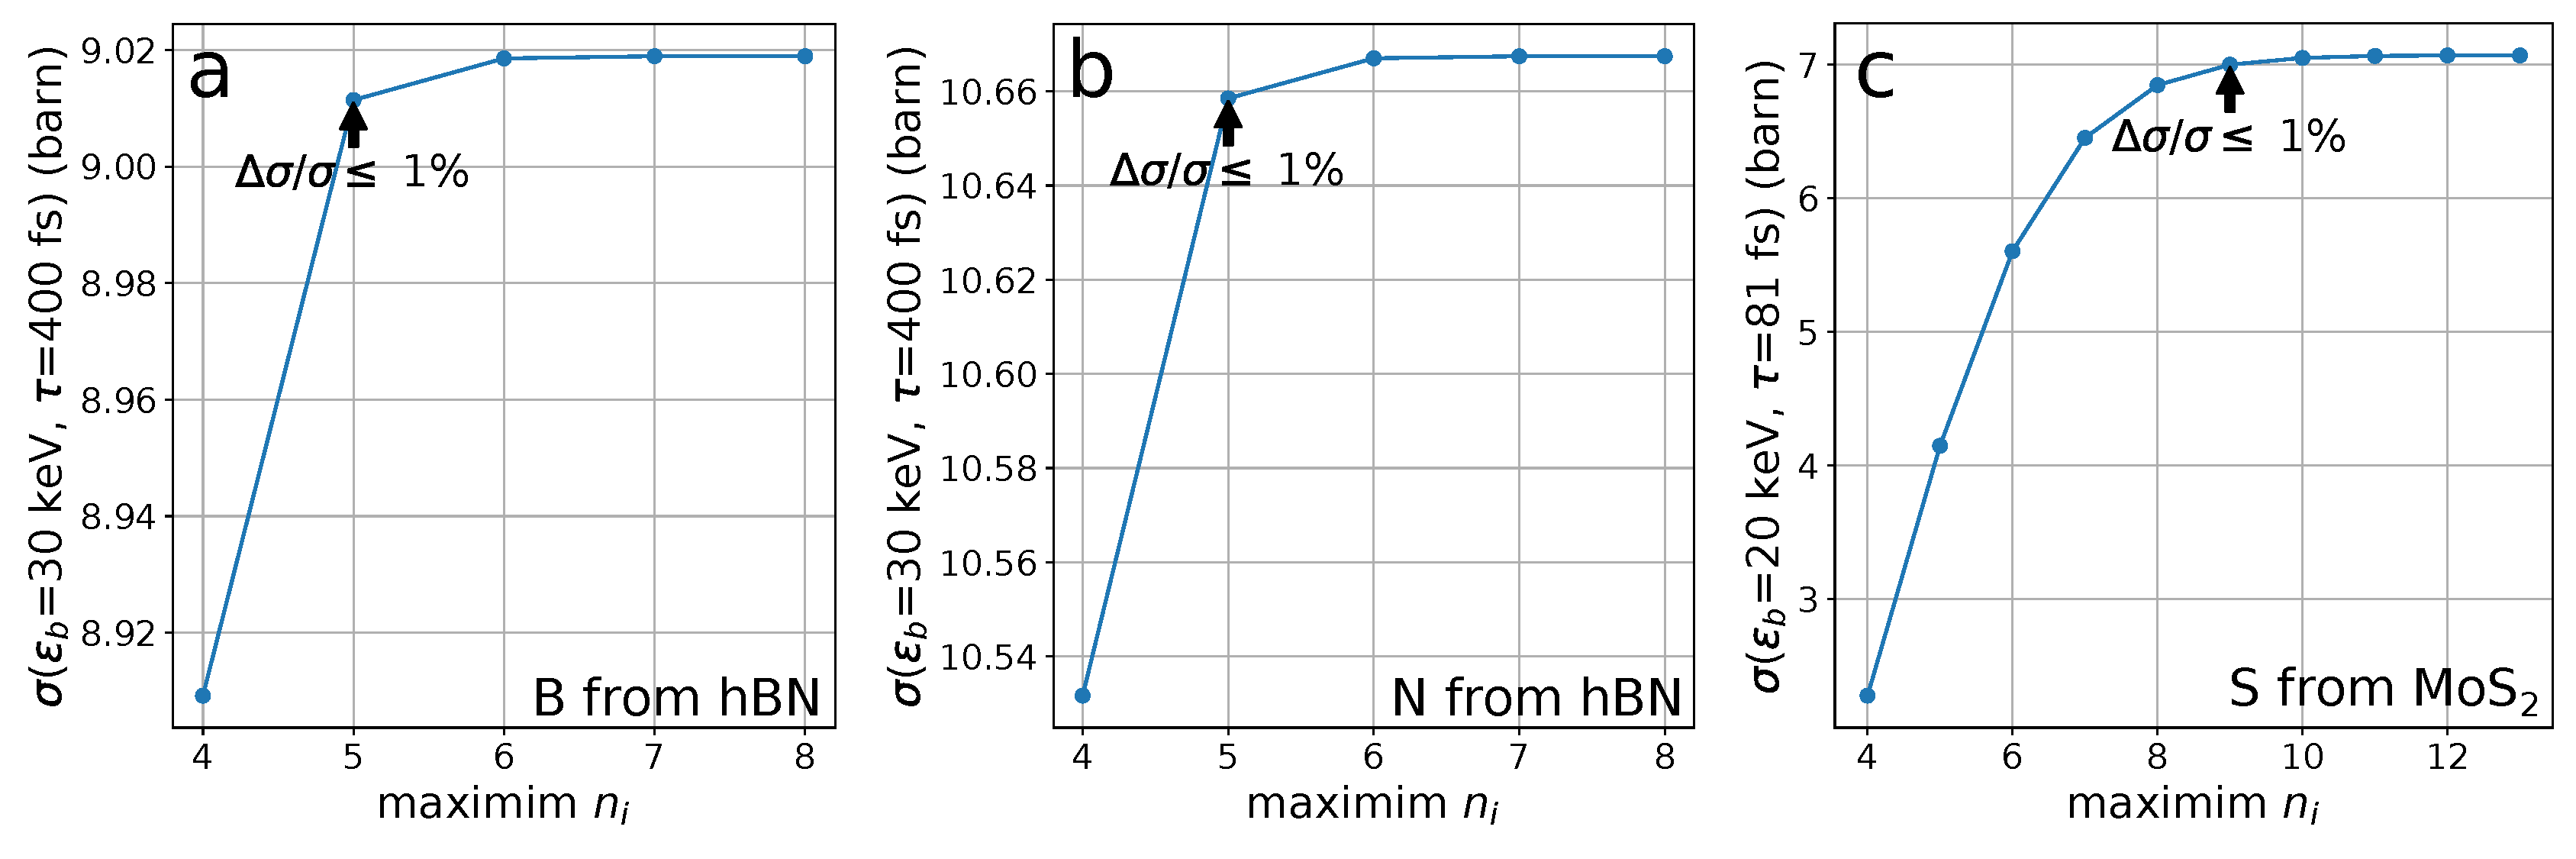
\includegraphics[width=\textwidth]{figS1.pdf}
  \caption{
    Convergence of the sputtering cross section with respect to the maximum
    number of beam-induced excitations $n_i^\text{max}$ considered.
    The simulated beam energies $\epsilon_b$ are the lowest experimental beam
    energies used for each material.
    The excitation lifetimes $\tau$ are those used to fit the experimental data
    in figures \ref{fig:edgeCross} and \ref{fig:MoS2Cross}.
    Each cross section is deemed converged when any increase in $n_i^\text{max}$
    increases the cross section by less than 1\%.
  }
  \label{fig:nimax}
\end{figure}

%------------------------------------------------------------------------------
\pagebreak
\section{Peaks in the sputtering cross section of hBN}
\label{app:edgePeaks}
%------------------------------------------------------------------------------

\begin{figure}[H]
  \centering
  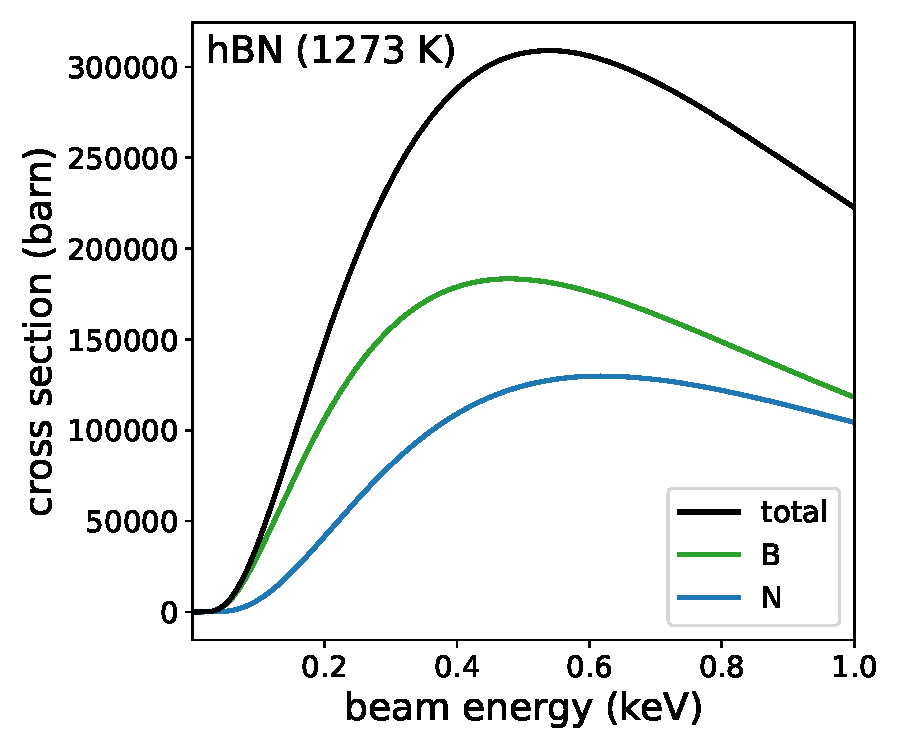
\includegraphics[width=0.6\textwidth]{figS2.pdf}
  \caption{
    The sputtering cross sections of boron and nitrogen from the hBN armchair
    edge peak at beam energies much lower than those typically used for
    microscopy and defect engineering.
    However, as mentioned in the main text, the validity of our perturbative
    approximation to the scattering operator breaks down at low beam energies
    (section \ref{sec:Pi}).
    Thus, the values and positions of these peaks may change if higher order
    perturbation terms are considered.
  }
  \label{fig:edgePeaks}
\end{figure}

%-------------------------------------------------------------------------------
\pagebreak
\section{Fitting and converging $S$}
\label{app:fitting}
%-------------------------------------------------------------------------------

\begin{figure}[H]
  \centering
  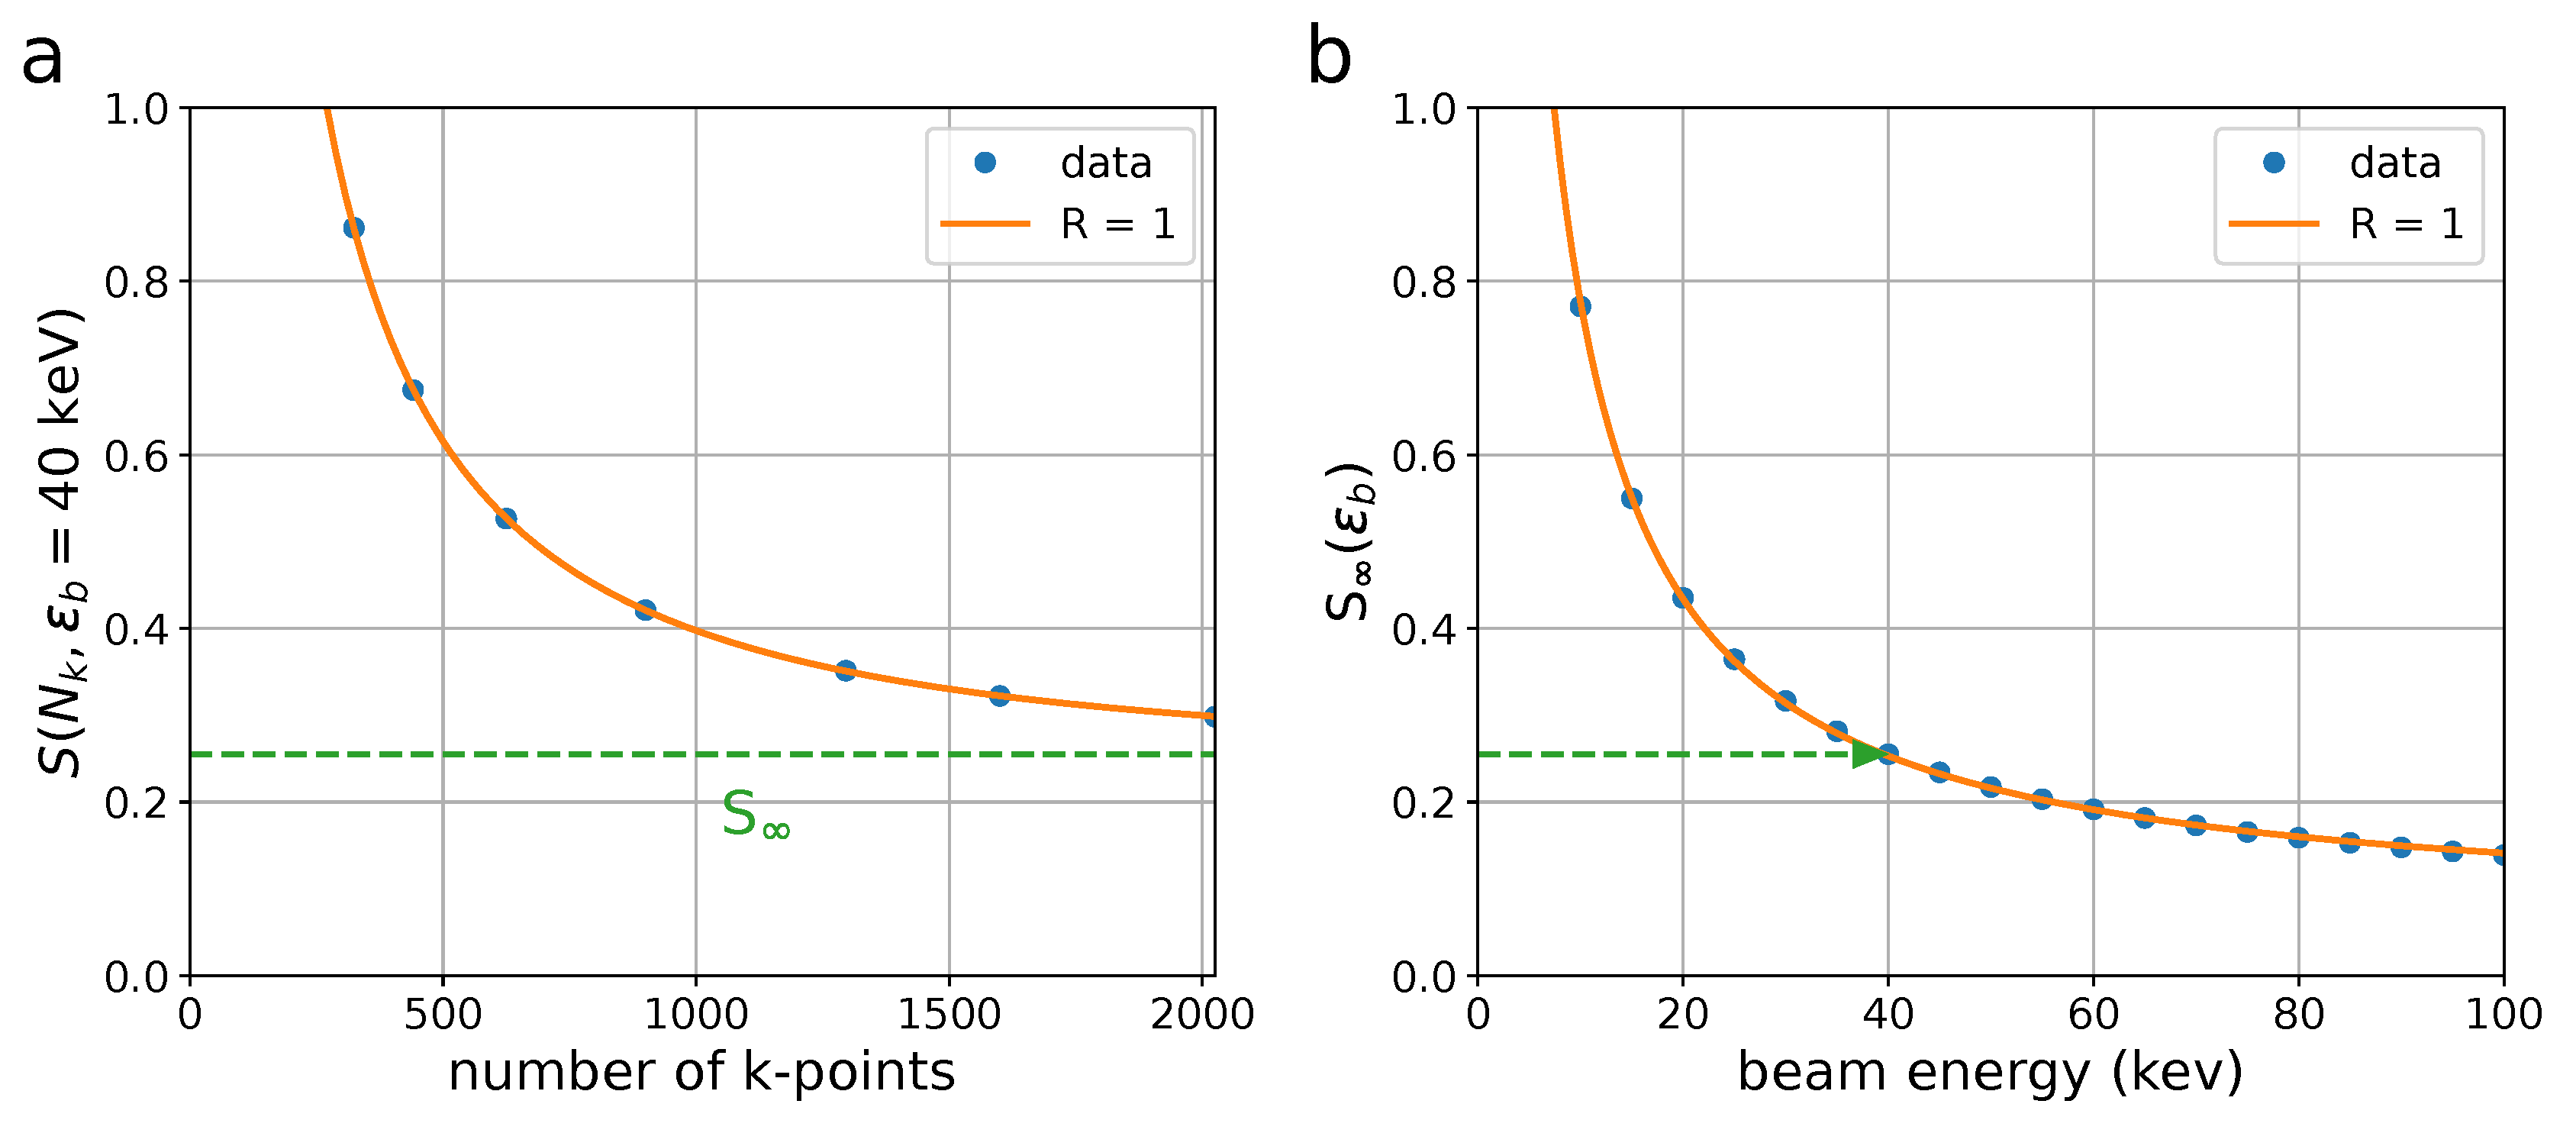
\includegraphics[width=\textwidth]{figS3.pdf}
  \caption{
    Finding the large crystal limit of $S(\epsilon_b)$ requires extrapolation.
    Panel (a) shows the dependence of $S$ on the number k-points $N_k$ in the
    Brillouin zone of hBN under 40 keV irradiation.
    The simulated points are fitted well by equation (\ref{eq:SNk}).
    The green dashed line denotes $S_\infty$, the asymptotic limit of $S(N_k)$
    for large $N_k$.
    Panel (b) then shows the dependence of $S_\infty$ on the beam energy
    $\epsilon_b$, which is fitted well by equation (\ref{eq:SEb}).
    The green arrow in panel (b) illustrates how $S_\infty(\epsilon_b=40\text{
    keV})$ is determined by the fit in panel (a).
  }
  \label{fig:Sfit}
\end{figure}

For a given beam energy $\epsilon_b$, we calculate the sum of all transition
probabilities $S$ defined in equation (\ref{eq:S}) for various k-point
densities where the number of k-points in the Brillouin zone is $N_k$.
We then fit the points to a curve of the form

\begin{equation}
  S(N_k, \epsilon_b)
  =
  \frac{a}{N_k-b}e^{-cN_k} + S_\infty,
  \label{eq:SNk}
\end{equation}
%
where $a$, $b$, $c$, and $S_\infty$ are all fitting parameters that depend on
$\epsilon_b$ (figure \ref{fig:Sfit}a).
We repeat this for multiple values of $\epsilon_b$ ranging from 5 to 100 keV
and record the best fit
$S_\infty$ for each
% and then use equation (\ref{eq:SNk}) to determine
$\epsilon_b$.
Based on the work of Bethe \cite{Bethe1930, Susi2019, Kretschmer2020}, we fit the resulting values of
$S_\infty(\epsilon_b)$ to an inverse function,

\begin{equation}
  S_\infty(\epsilon_b)
  =
  \frac{A}{\epsilon_b - B} + C.
  \label{eq:SEb}
\end{equation}
%
where $A$, $B$, and $C$ are fitting parameters.  The parameters for hBN and
MoS$_2$ are given in table \ref{tab:fit}.
The fitted curve can then be substituted for $S(\epsilon_b)$ in formula
(\ref{eq:Pi}) to obtain $P_i(\epsilon_b, n_i)$, the probability of exciting
$n_i$ electrons in the large crystal limit.

\begin{table} \centering 
  \begin{tabular}{lccc}
    \toprule
    material &A (eV) &B (eV) &C \\
    \midrule
    hBN     &7.655 &-0.770 &0.06526 \\
    MoS$_2$ &49.05 &-3.867 &0.3547 \\
    \bottomrule
  \end{tabular}
  \caption{
    Fitting parameters of equation (\ref{eq:SEb}) for hBN and MoS$_2$.
  } 
\label{tab:fit}
\end{table}

Finally, $S$ must also be converged with respect all parameters.  These include
the maximum virtual photon momentum, DFT cutoff energy, and height of the
pristine unit cell (figure \ref{fig:convergences}).
$S$ is considered converged with respect to a parameter when any increase in
the parameter's precision changes $S$ by less than 5\%.

\begin{figure}[H]
  \centering
  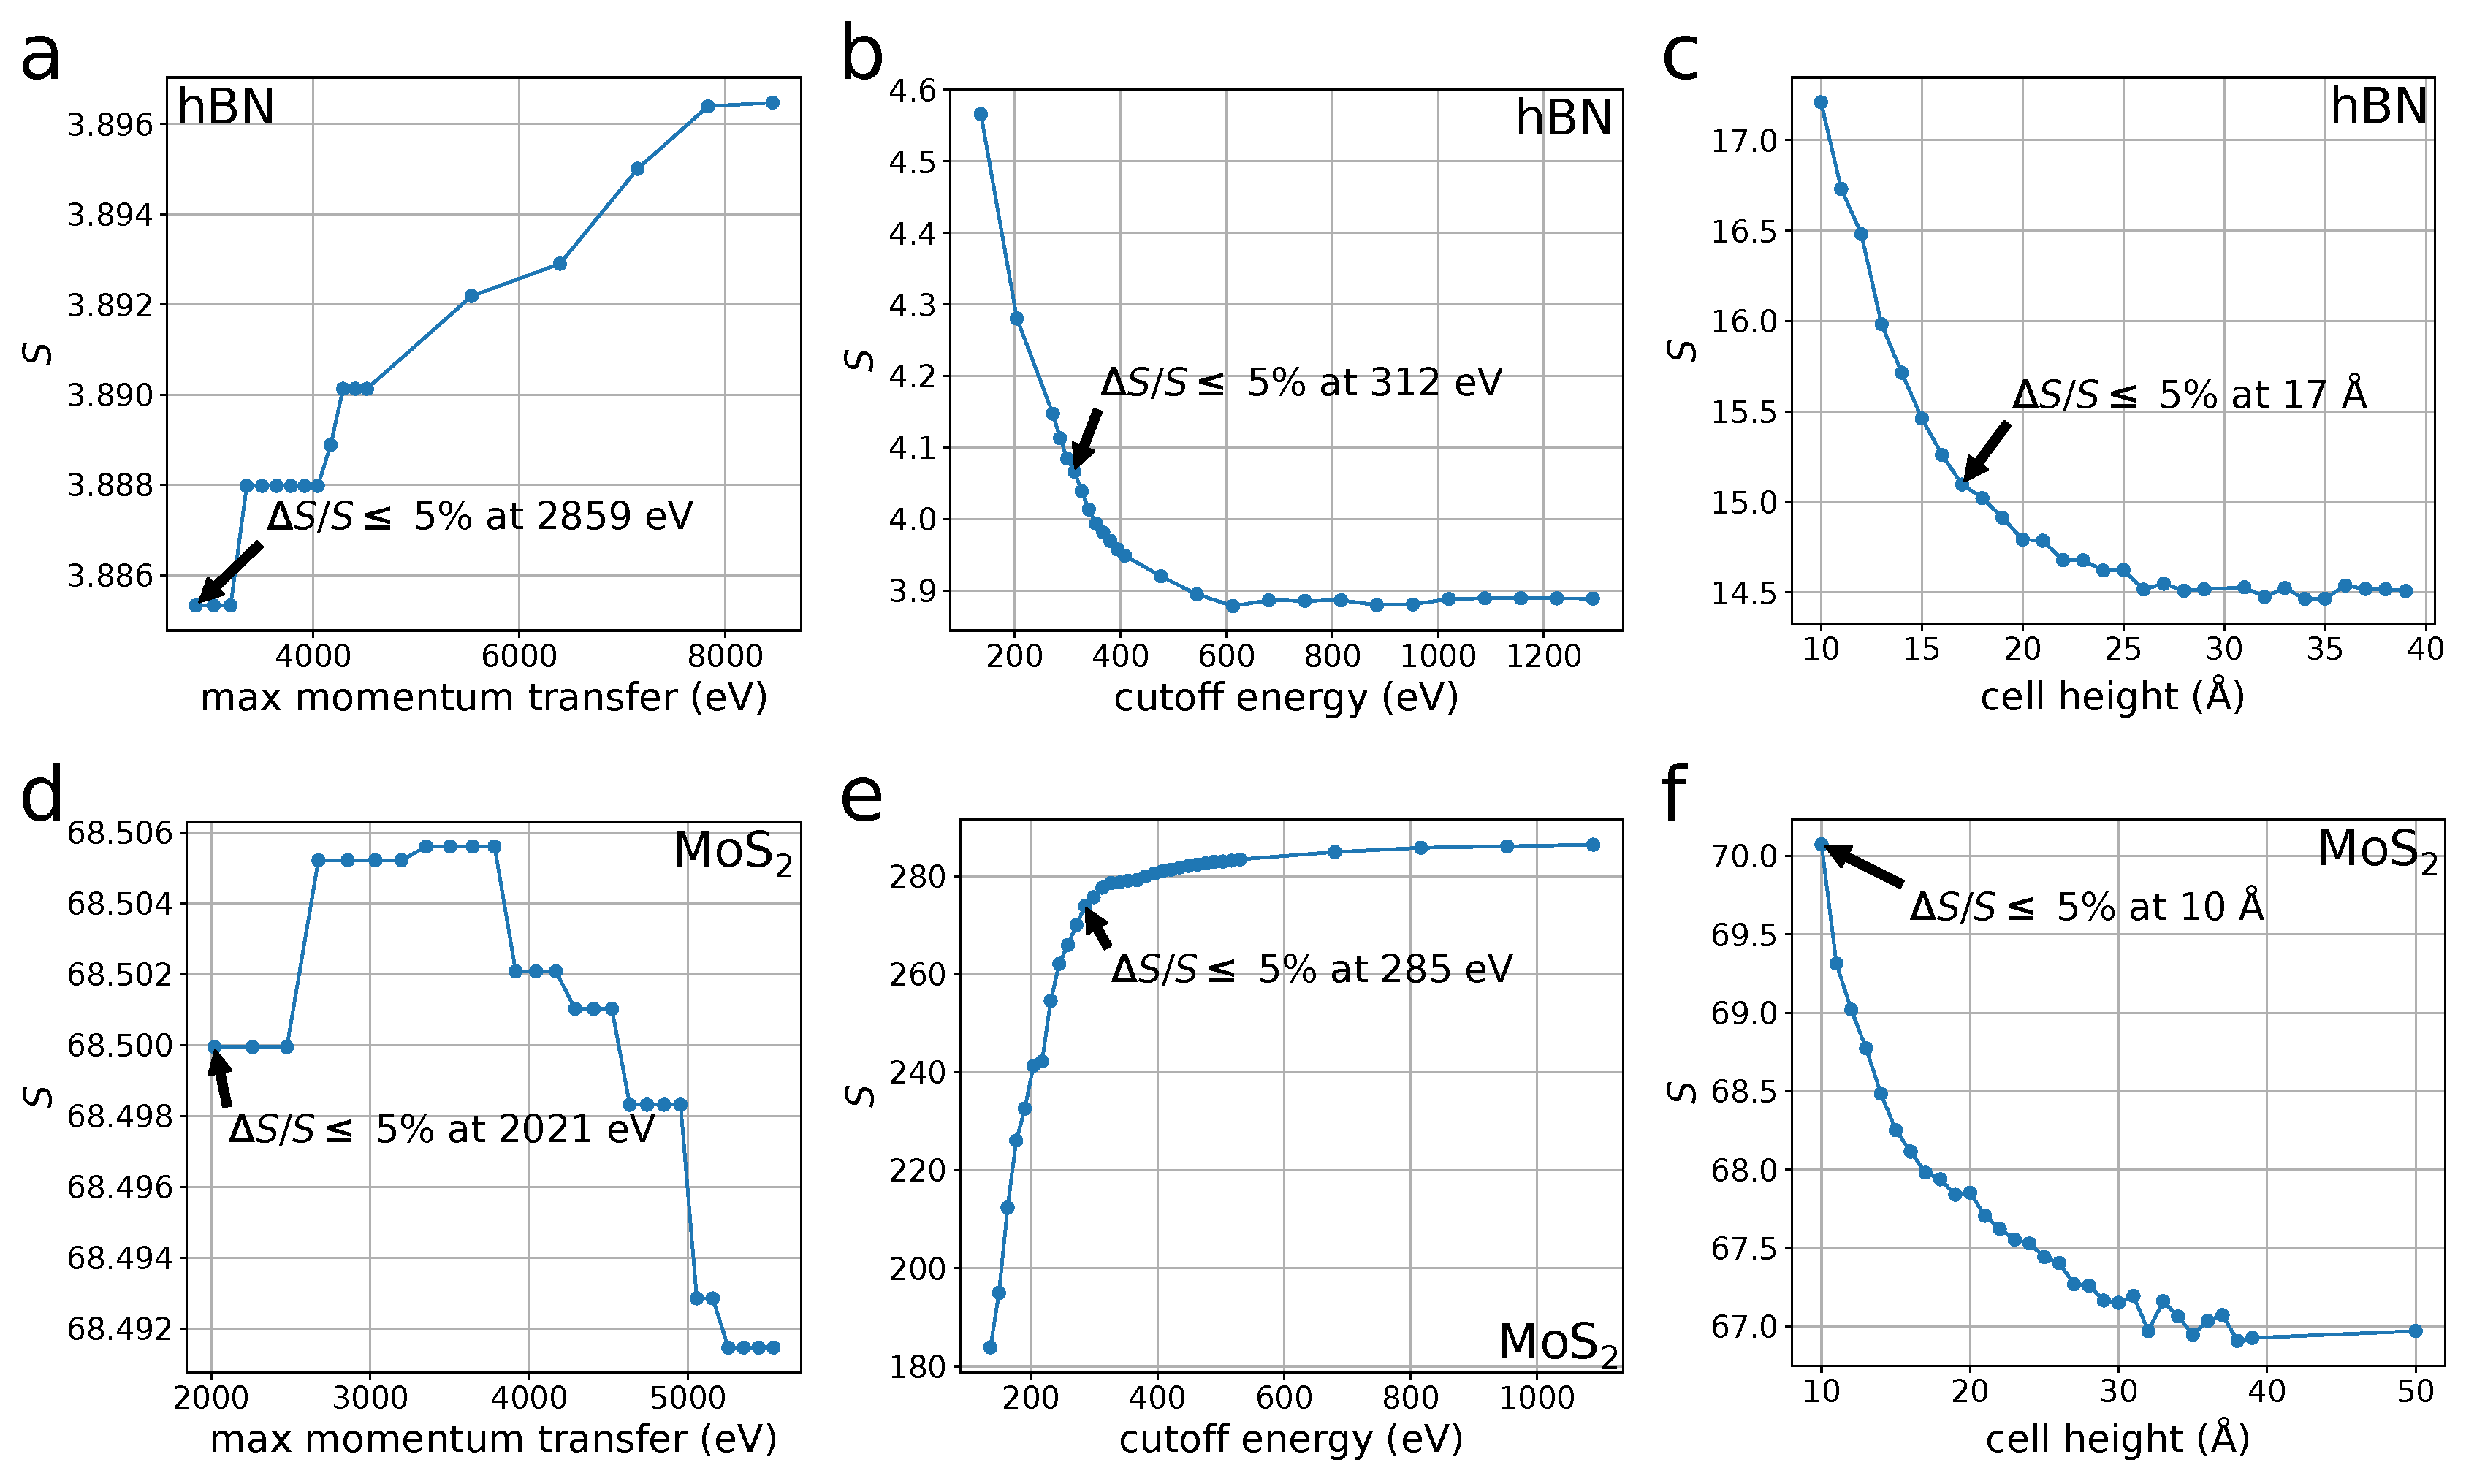
\includegraphics[width=\textwidth]{figS4.pdf}
  \caption{
    Convergence of $S$ with respect to the (a and d) maximum magnitude of
    virtual photon momentum considered, (b and e) plane-wave DFT cutoff energy,
    and (c and f) height of the unit cell.
    A $6\times6\times1$ k-point mesh and a beam energy of 60 keV is used to
    generate all six plots.
    The converged parameters were found to be insensitive to changes in k-point
    density and beam energy.
    $S$ is deemed converged when any increase in precision changes $S$ by less
    than 5\%.
  }
  \label{fig:convergences}
\end{figure}
\break

%------------------------------------------------------------------------------
\pagebreak
\section{Calculating $E_\text{min}$}
\label{app:Emin}
%------------------------------------------------------------------------------

\begin{figure}[H]
  \centering
  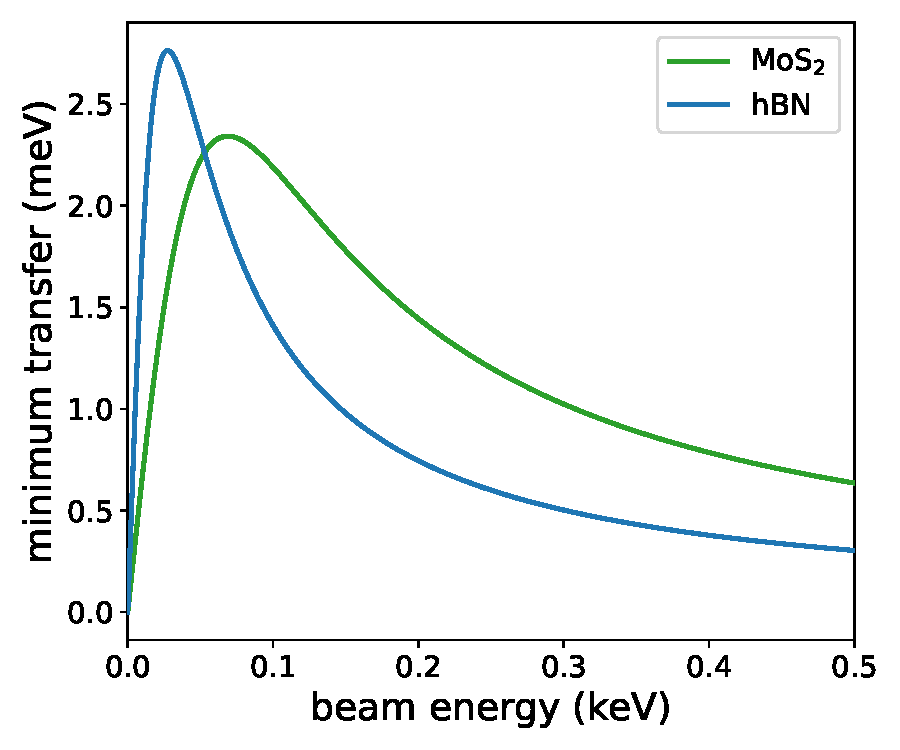
\includegraphics[width=0.6\textwidth]{figS5.pdf}
  \caption{
    The minimum energy transfer from the beam electron to the target nucleus
    peaks at very low beam energies and is always much smaller than the
    nuclei's average thermal kinetic energy of $\sim$39 meV at room
    temperature. 
  }
  \label{fig:Emin}
\end{figure}

In hBN, a unit cell contains a boron and nitrogen atom.
As these atoms have similar masses and displacement thresholds (table
\ref{tab:Ed}), the sputtering of both atoms should be considered for a given
beam energy.
Thus, we approximate the maximum cross sectional area $\sigma_\text{max}$ of
these atoms to be $\Omega_\text{hBN}/2$, where $\Omega_\text{hBN}$ is the area
of the hBN unit cell.
On the other hand, molybdenum is much heavier than sulfur and has a much larger
displacement threshold in MoS$_2$ \cite{Komsa2012}.  
This means that only the sputtering of sulfur needs to be considered.
Additionally, of the two sulfur atoms in the MoS$_2$ unit cell, only the atom
on the outgoing surface is eligible to sputter from a pristine system
\cite{Komsa2012}.
Therefore, $\sigma_\text{max}$ for sulfur sputtering from MoS$_2$ is
$\Omega_\text{MoS$_2$}$, the area of the MoS$_2$ unit cell.

To approximate $E_\text{min}$, we use the Rutherford displacement cross section
\cite{Thornton2004, Sakurai2011, Yoshimura2018} as an approximation to equation
(\ref{eq:basicSigma}),

\begin{equation}
  \sigma_R
  =
  \pi\left(\frac{Z\alpha}{|\mathbf{p}|\beta}\right)^2
  \left(\frac{E_\text{max}}{E_d} - 1\right).
  \label{eq:Rutherford}
\end{equation}
%
Setting $\sigma_R=\sigma_\text{max}$ and $E_d=E_\text{min}$ and solving for
$E_\text{min}$ yields

\begin{equation}
  E_\text{min}(\epsilon_b)
  =
  E_\text{max}
  \left[\frac{\Omega}{\pi}
    \left(\frac{|\mathbf{p}_b|\beta}{Z\alpha}\right)^2 + 1
  \right]^{-1}.
  \label{eq:Emin}
\end{equation}
%
Using the Rutherford cross section instead of the McKinley-Feshbach
cross section should be accurate for small beam energies for which $\beta\ll
1$.
This makes it well-suited for finding $E_\text{min}$, since
$E_d(n_f)<E_\text{min}$ only for large $n_f$, and large $n_i$ (and thus $n_f$)
are much more likely for small beam energies (figure \ref{fig:Pi}).

With that said, the sputtering cross section is fairly insensitive to the exact
value of $E_\text{min}$ when $E_\text{min} \ll E_\text{max}$.
This is because the post-collision velocity of the PKA diminishes when the
energy transfer $E$ shrinks.
The beam-induced excitations therefore have more time to relax before the PKA
reaches the step in the energy surface (section \ref{sec:assumptions}).
This makes $P_f$ small for small $E$, so that contributions to the integral in
equation (\ref{eq:totSigma}) are extremely tiny for $E$ near $E_\text{min}$.
As a result, changes in $E_\text{min}$ are essentially immeasurable for beam
energies greater than 1 keV.
Nonetheless, the use of $E_\text{min}$ is necessary for the calculation of a
finite sputtering cross section.


\bibliography{library}
\bibliographystyle{ieeetr}

\end{document}

% %-------------------------------------------------------------------------------
% \section{Interaction Hamiltonian and the scattering operator}
% \label{app:S}
% %-------------------------------------------------------------------------------
% 
% For the case of electron beam-matter scattering, the probability of a
% particular scattering event can be calculated by taking the time-evolution of
% the incident electron state(s) in the presence of the electromagnetic field
% interaction and determining overlap of the time-evolved state(s) with the final
% state(s) of interest. In the interaction picture of quantum mechanics, this
% time-evolution is governed by the interaction term in the Hamiltonian
% \cite{Sakurai2011}.  We therefore begin this chapter by deriving this term.  As
% a starting point, assuming units in which $\hbar = c = 1$, the noninteracting
% Lagrangian density of the electromagnetic and electron fields is
% 
% \begin{equation}
% \label{eq:nonIntL}
%     \hat{\mathcal{L}}
%     =
%     -\frac{1}{4}\hat{F}_{\mu\nu}\hat{F}^{\mu\nu}
%     +
%     \hat{\bar{\psi}}(i\gamma^\mu \partial_\mu - m)\hat{\psi},
% \end{equation}
% %
% where the electromagnetic vector field operator can be expressed as
% 
% \begin{equation}
%     \hat{A}_\mu(x)
%     =
%     \int\frac{d^3q}{(2\pi)^{3/2}}\frac{1}{(2E_\mathbf{q})^{1/2}}
%     \sum_{\lambda=1}^2
%     \left(
%     \hat{c}_{\lambda\mathbf{q}}\epsilon^\lambda_\mu(q)e^{-iq\cdot x}
%     +
%     \hat{c}^\dag_{\lambda\mathbf{q}}\epsilon^{\lambda*}_\mu(q)e^{iq\cdot x}
%     \right),
% \end{equation}
% %
% where $E_\mathbf{q}^2 = |\mathbf{q}|^2$, $\epsilon^\lambda_\mu$ are the
% polarization vectors for polarizations $\lambda=1$ or 2, and the raising and
% lower operators obey the commutation relations
% 
% \begin{equation}
%     [\hat{c}_{\lambda\mathbf{p}}, \hat{c}^\dag_{\lambda'\mathbf{p}'}]
%     =
%     \delta(\mathbf{p} - \mathbf{p'})\delta_{\lambda\lambda'}.
% \end{equation}
% %
% With this, the electromagnetic tensor field operator is
% 
% \begin{equation}
%     \hat{F}_{\mu\nu} = (\partial_\mu \hat{A}_\nu - \partial_\nu \hat{A}_\mu).
% \end{equation}
% %
% In the electron term, the $\gamma^\mu$ matrices are a set of $4\times4$
% matrices that satisfy the anticommutation relations
% 
% \begin{equation}
%     \{\gamma^\mu, \gamma^\nu\} = 2g^{\mu\nu},
% \end{equation}
% %
% where $g^{\mu\nu}$ is the metric tensor of Minkowski, so that
% 
% \begin{equation}
%     g^{\mu\nu} 
%     =
%     \mqty(
%     1&0&0&0\\
%     0&-1&0&0\\
%     0&0&-1&0\\
%     0&0&0&-1
%     ).
% \end{equation}
% %
% Further, the electron spinor field operators can be expressed as
% 
% \begin{equation}
% \label{eq:electronField}
% \begin{aligned}
%     &\hat{\psi}(x)
%     =
%     \int\frac{d^3p}{(2\pi)^{3/2}}\frac{1}{(2\epsilon_\mathbf{p})^{1/2}}
%     \sum_{s=1}^2
%     \left(
%     \hat{a}_{s\mathbf{p}}u^s(p)e^{-ip\cdot x}
%     +
%     \hat{b}^\dag_{s\mathbf{p}} v^s(p)e^{ip\cdot x}
%     \right)
%     \\&\hat{\bar{\psi}}(x)
%     =
%     \int\frac{d^3p}{(2\pi)^{3/2}}\frac{1}{(2\epsilon_\mathbf{p})^{1/2}}
%     \sum_{s=1}^2
%     \left(
%     \hat{a}^\dag_{s\mathbf{p}} \bar{u}^s(p)e^{-ip\cdot x}
%     +
%     \hat{b}_{s\mathbf{p}} \bar{v}^s(p)e^{ip\cdot x}
% \right),
% \end{aligned}
% \end{equation}
% %
% where $\epsilon_\mathbf{p} = |\mathbf{p}|^2 + m^2$, $u^s(p)$ and $v^s(p)$ are
% spinors for spin component $s$, $\bar{u}(p) = u^\dag(p)\gamma^0$, and the
% raising and lowering operators obey the anticommutation relations
% 
% \begin{equation}
%     \{\hat{a}_{s\mathbf{p}}, \hat{a}^\dag_{r\mathbf{q}}\}
%     =
%     \{\hat{b}_{s\mathbf{p}}, \hat{b}^\dag_{r\mathbf{q}}\}
%     =
%     \delta(\mathbf{p} - \mathbf{q})\delta_{sr}.
% \end{equation}
% %
% As written, both fields in equation (\ref{eq:nonIntL}) are and will always be
% completely stationary. Any dynamics in these fields require addition of an
% interaction term in the Lagrangian density.  The precise form of this term
% follows directly from gauge invariance.  We know that electromagnetism is gauge
% invariant, in that changes to the vector field of the form
% 
% \begin{equation}
% \label{eq:emGauge}
%     A_\mu \rightarrow A_\mu-q^{-1}\partial_\mu \alpha(x)
%     \quad
%     \Rightarrow
%     \quad
%     F_{\mu\nu} \rightarrow F_{\mu\nu}
% \end{equation}
% %
% leave the tensor field unchanged.  As the tensor field is what is actually
% measured, there should be no way to experimentally detect a change of this form
% in the vector field.  With that said, we also know from the Aharonov-Bohm effect
% \cite{Aharonov1959} that the transformation in (\ref{eq:emGauge}) results in a
% local phase change to the electron field, specifically
% 
% \begin{equation}
%     \label{eq:aharonov}
%     \psi\rightarrow\psi e^{i\alpha(x)}.
% \end{equation}
% %
% (Note the fact that a charged field must transform like this guarantees that it
% is complex).  Thus, for our theory to remain gauge invariant, it follows that
% the Lagrangian in equation (\ref{eq:nonIntL}) must be invariant to both
% (\ref{eq:emGauge}) and (\ref{eq:aharonov}).  With this provision, let us check
% if the noninteracting Lagrangian as written in equation (\ref{eq:nonIntL}) is
% indeed gauge invariant.  Clearly, relation (\ref{eq:emGauge}) states that the
% electromagnetic term remains unchanged.  Meanwhile, to check the electron term,
% we can multiply out the contents in parenthesis and check the two terms
% individually.  While it is easy to see that mass term is gauge invariant, the
% derivative term is not, in that
% 
% \begin{equation}
% \label{eq:derTerm}
%     \bar{\psi}\partial_\mu\psi
%     \rightarrow
%     \bar{\psi}\partial_\mu\psi + i\bar{\psi}\psi\partial_\mu\alpha(x)
%     \neq
%     \bar{\psi}\partial_\mu\psi.
% \end{equation}
% %
% Therefore, a term must be added to equation (\ref{eq:nonIntL}) to make it gauge
% invariant.  The hope is that this term, when transformed by (\ref{eq:emGauge}),
% will cancel the extra term containing $\alpha(x)$ in (\ref{eq:derTerm}).  For
% this, we can replace the derivative with a covariant derivative
% 
% \begin{equation}
%     \label{eq:covDer}
%     D_\mu = \partial_\mu + iqA_\mu.
% \end{equation}
% %
% In doing so, the electron term in the Lagrangian now gauge transforms like
% 
% \begin{equation}
%     \begin{aligned}
% \bar{\psi}D_\mu\psi
% &=
% \bar{\psi}\partial_\mu\psi + iq\bar{\psi}A_\mu\psi
% \\&\rightarrow
% \bar{\psi}\partial_\mu\psi + i\bar{\psi}\psi\partial_\mu\alpha
% +
% iq\bar{\psi}A_\mu\psi - i\bar{\psi}\psi\partial_\mu\alpha
% \\&=
% \bar{\psi}\partial_\mu\psi + iq\bar{\psi}A_\mu\psi
% =
% \bar{\psi}D_\mu\psi.
% \end{aligned}
% \end{equation}
% %
% Thus, we see that replacing the derivative with the covariant derivative makes
% the Lagrangian gauge invariant.
% 
% If we isolate the change in the Lagrangian density due to the inclusion of the
% covariant derivative, we obtain the noninteracting Lagrangian density plus an
% extra term
% 
% \begin{equation}
%     \mathcal{L}
%     =
%     -\frac{1}{4}F_{\mu\nu}F^{\mu\nu}
%     +
%     \bar{\psi}(i\gamma^\mu \partial_\mu - m)\psi - q\bar{\psi}\gamma^\mu A_\mu\psi.
% \end{equation}
% %
% In doing so, we see that the last term is the interaction Lagrangian density,
% the negative of which is the interacting Hamiltonian density
% 
% \begin{equation}
%     \label{eq:Hi}
%     \hat{\mathcal{H}}_I = q\hat{\bar{\psi}}\gamma^\mu \hat{A}_\mu\hat{\psi},
% \end{equation}
% %
% where we now interpret $q$ as the electromagnetic charge.  As stated before, in
% the interaction picture, the interacting Hamiltonian dictates how quantum
% states evolve in time through the time-evolution operator
% 
% \begin{equation}
%     \hat{S}=T\left[\exp\left(-i\int d^4x\hat{\mathcal{H}}_I(x)\right)\right],
%     \label{eq:Shat}
% \end{equation}
% %
% where $T$ is the time-ordering operator.  This operator is the key ingredient
% for calculating scattering cross sections, as it allows us to determine the
% probability amplitude for the evolution of any state into another.
% 
% The amplitude density for two free electrons of momenta $p_1$ and $p_2$ to
% scatter into states $p_3$ and $p_4$ is given by the sandwiching the scattering
% operator $\hat{S}$ defined in equation (\ref{eq:Shat}) between the initial and
% final free-particle states, so that
% 
% \begin{equation}
% \label{eq:SExpansion}
%     \begin{aligned}
%     \bra{p_4 p_3}\hat{S}\ket{p_2p_1}
%     &=
%     \bra{p_4p_3} \ket{p_2p_1}
%     \\&-
%     \frac{1}{2} \int d^4x d^4y
%     \bra{p_4p_3} \hat{\mathcal{H}}_I(x)\hat{\mathcal{H}}_I(y)\ket{p_2p_1}
%     \\&+
%     \mathcal{O}(e^4).
% \end{aligned}
% \end{equation}
% %
% The first term in the expansion describes the case of no interaction between
% the particles.  Beyond this, Wick's theorem dictates that all odd-order terms
% vanish.  We therefore use the second order term to approximate the scattering
% amplitude.
% % Higher order terms are of the order $\mathcal{O}(e^4\ll 1)$ and can be ignored.
% Using the form of the interaction Hamiltonian density in equation
% (\ref{eq:Hi}), we define the scattering amplitude as
% 
% \begin{equation}
% \label{eq:mollerContraction}
% \begin{aligned}
%     \bra{p_4p_3}&\hat{T}\ket{p_2p_1}
%     \equiv
%     -\frac{1}{2} \int d^4x d^4y
%     \bra{p_4p_3} \hat{\mathcal{H}}_I(x)\hat{\mathcal{H}}_I(y)\ket{p_2p_1}
%     \\&=
%     -\frac{e^2}{2}\int d^4x d^4y
%     \bra{p_4p_3}
%     \hat{\bar{\psi}}(x)\gamma^\mu A_\mu(x) \hat{\psi}(x)
%     \hat{\bar{\psi}}(y)\gamma^\nu A_\nu(y) \hat{\psi}(y)
%     \ket{p_2p_1}
%     \\&=
%     e^2\int d^4x d^4y\bigg\{
%     \contraction[1ex]
%         {\langle}{\hat{\bar{p}}_4}{p_3|}{\hat{\bar{\psi}}(x)}
%     \contraction[2ex]
%         {\langle p_4}{\bar{\psi}_3}
%         {|\hat{\bar{\psi}}(x)\gamma^\mu A_\mu(x)\hat{\psi}(x)}
%         {\bar{\hat{\psi}}(y)}
%     \contraction[1ex]
%         {\bra{p_4p_3}
%         \hat{\bar{\psi}}(x)\gamma^\mu}{A_\mu(x)}
%         {\hat{\psi}(x) \hat{\bar{\psi}}(y)\gamma^\nu}{A_\nu(y)}
%     \bcontraction[1ex]
%         {\bra{p_4p_3}
%         \hat{\bar{\psi}}(x)\gamma^\mu A_\mu(x)}{\hat{\psi}(}
%         {x)\hat{\bar{\psi}}(y)\gamma^\nu A_\nu(y) \hat{\psi}(y)||p_2}
%         {p}
%     \contraction[1ex]
%         {\bra{p_4p_3}
%         \hat{\bar{\psi}}(x)\gamma^\mu A_\mu(x) \hat{\psi}(x)
%         \hat{\bar{\psi}}(y)\gamma^\nu A_\nu(y)}{\hat{w}(y)}
%         {}{|p_2}
%     \bra{p_4p_3}
%     \hat{\bar{\psi}}(x)\gamma^\mu A_\mu(x) \hat{\psi}(x)
%     \hat{\bar{\psi}}(y)\gamma^\nu A_\nu(y) \hat{\psi}(y)
%     \ket{p_2p_1}
%     \\&\qquad\qquad\quad+
%     \contraction[2ex]
%         {\langle}{\hat{\bar{p}}_4} {p_3|
%         \hat{\bar{\psi}}(x)\gamma^\mu A_\mu(x) \hat{\psi}(x)}
%         {\hat{\bar{\psi}}(y)}
%     \contraction[1ex]
%         {\langle p_4}{\bar{\psi}_3}{}
%         {|\hat{\bar{\psi}}(x)}
%     \contraction[1ex]
%         {\bra{p_4p_3}
%         \hat{\bar{\psi}}(x)\gamma^\mu}{A_\mu(x)}
%         {\hat{\psi}(x) \hat{\bar{\psi}}(y)\gamma^\nu}{A_\nu(y)}
%     \bcontraction[1ex]
%         {\bra{p_4p_3}
%         \hat{\bar{\psi}}(x)\gamma^\mu A_\mu(x)}{\hat{\psi}(}
%         {x)\hat{\bar{\psi}}(y)\gamma^\nu A_\nu(y) \hat{\psi}(y)||p_2}
%         {p}
%     \contraction[1ex]
%         {\bra{p_4p_3}
%         \hat{\bar{\psi}}(x)\gamma^\mu A_\mu(x) \hat{\psi}(x)
%         \hat{\bar{\psi}}(y)\gamma^\nu A_\nu(y)}{\hat{w}(y)}
%         {}{|p_2}
%     \bra{p_4p_3}
%     \hat{\bar{\psi}}(x)\gamma^\mu A_\mu(x) \hat{\psi}(x)
%     \hat{\bar{\psi}}(y)\gamma^\nu A_\nu(y) \hat{\psi}(y)
%     \ket{p_2p_1}
%     \bigg\}.
% \end{aligned}
% \end{equation}
% %
% The scattering amplitude is then related to the invariant matrix element
% $\mathcal{M}$ by equation (\ref{eq:amp}) in the main text.
% 
% 
% %------------------------------------------------------------------
% \section{Wick's Theorem}
% \label{app:wicks}
% %------------------------------------------------------------------
% 
% Wick's theorem allows us to express the long strings of time-ordered operators
% generated from the expansion of the S-matrix in terms of free particle
% propagators \cite{Lancaster2014, Peskin1995}.  In our study of scattering, for
% which the initial and final states are chosen to be those of asymptotically
% noninteracting particles, these strings of operators are sandwiched between
% momentum eigenstates, and can be written as
% 
% \begin{equation}
%     \bra{\mathbf{p}_1, \mathbf{p}_2, ...}
%     T[\hat{A}\hat{B}\hat{C}...]
%     \ket{\mathbf{q}_1, \mathbf{q}_2, ...}
%     =
%     \bra{0}
%     T[
%     \hat{a}_{\mathbf{p}_1}
%     \hat{a}_{\mathbf{p}_2}
%     ...
%     \hat{A}\hat{B}\hat{C}...
%     \hat{a}_{\mathbf{q}_1}^\dag
%     \hat{a}_{\mathbf{q}_2}^\dag
%     ...
%     ]
%     \ket{0}.
% \end{equation}
% %
% The term on the right, being sandwiched by noninteracting vacuum states, is
% called a vacuum expectation value (VEV).  VEVs of time-ordered operators are at
% first not easy to solve.  In contrast, the VEVs of normal-ordered operators, in
% which all creation operators are written to the right of the annihilation
% operators, are easily shown to be zero. That is,
% 
% \begin{equation}
%     \bra{0}
%     N[
%     \hat{a}_{\mathbf{p}_1}
%     \hat{a}_{\mathbf{p}_2}
%     ...
%     \hat{A}\hat{B}\hat{C}...
%     \hat{a}_{\mathbf{q}_1}^\dag
%     \hat{a}_{\mathbf{q}_2}^\dag
%     ...
%     ]
%     \ket{0}
%     =
%     0,
% \end{equation}
% %
% where $N$ is the normal-ordering operator.
% This is because the vacuum ket is preceded by annihilation operators and/or the
% vacuum bra is superseded by creation operators.  We define the contraction of
% two operators as 
% 
% \begin{equation}
%     \label{eq:contraction}
%     \contraction[1ex]
%         {}{\hat{A}}{}{B}
%         \hat{A}\hat{B}
%     =
%     T[\hat{A}\hat{B}]
%     -
%     N[\hat{A}\hat{B}].
% \end{equation}
% %
% Note that the contraction is a number, not an operator, meaning that the VEV of
% a contraction is just the contraction itself.  From equation
% \ref{eq:contraction}, it can be shown that (see Peskin and Schroeder
% \cite{Peskin1995})
% 
% \begin{equation}
%     T[\hat{A}\hat{B}\hat{C}...]
%     =
%     N[\hat{A}\hat{B}\hat{C}...
%     +
%     \text{all possible contractions of }
%     \hat{A}\hat{B}\hat{C}...].
% \end{equation}
% %
% Taking the VEV of the right side would only leave terms which are fully
% contracted, in which all operators are contracted with another.  This is
% becuase any VEV containing uncontracted operators would vanish due to their
% normal ordering.  Thus, we can see that the VEV of a time-ordered product is
% the sum of all fully contracted terms.
% 
% The scattering amplitude given in equation (\ref{eq:mollerContraction})
% contains only two types of contractions.  The first is
% 
% \begin{equation}
% \begin{aligned}
%     \contraction[1ex]
%         {\bra{0}}{\hat{\psi}(x)}{}{\ket{p}}
%     \bra{0}\hat{\psi}(x)\ket{p}
%     &=
%     \contraction[1ex]
%         {(2\pi)^{3/2}(2\epsilon_\mathbf{p})^{1/2}\bra{0}}
%         {\hat{\psi}(x)}{}{\hat{a}^\dag}
%     (2\pi)^{3/2}(2\epsilon_\mathbf{p})^{1/2}
%     \bra{0}\hat{\psi}(x)\hat{a}^\dag_{s\mathbf{p}}\ket{0}
%     \\&=
%     (2\pi)^{3/2}(2\epsilon_\mathbf{p})^{1/2}
%     \bra{0}T[\hat{\psi}(x)\hat{a}^\dag_{s'\mathbf{p'}}]\ket{0}
%     \\&=
%     (2\pi)^{3/2}(2\epsilon_\mathbf{p})^{1/2}
%     \bra{0}
%     \int\frac{d^3q}{(2\pi)^{3/2}}
%     \frac{1}{(2\epsilon_\mathbf{q})^{1/2}}
%     \\&\quad\qquad\times
%     \sum_{r} \left(
%     u^{r}(q)\hat{a}_{r\mathbf{q}}e^{-iq\cdot x}
%     +
%     v^{r}(q)\hat{b}^\dag_{r\mathbf{q}}e^{iq\cdot x}
%     \right)
%     \hat{a}^\dag_{sp}
%     \ket{0}
%     \\&=
%     (2\pi)^{3/2}(2\epsilon_\mathbf{p})^{1/2}
%     \int\frac{d^3q}{(2\pi)^{3/2}}
%     \frac{1}{(2\epsilon_\mathbf{q})^{1/2}}
%     \sum_{r} 
%     u^{r}(q)e^{-iq\cdot x}
%     \delta(\mathbf{q-p})\delta_{rs}
%     \\&=
%     u^{s}(p)e^{-ip\cdot x}.
% \end{aligned}
% \end{equation}
% %
% The second is
% 
% \begin{equation}
%     \contraction[1ex]
%         {}{\hat{A}_\mu(x)}{}{\hat{A}_\nu(y)}
%     \hat{A}_\mu(x)\hat{A}_\nu(y)
%     =
%     \bra{0}
%     T[\hat{A}_\mu(x)\hat{A}_\nu(y)]
%     \ket{0}
%     \equiv
%     D_{0\mu\nu}(x, y),
% \end{equation}
% %
% which we recognize as the free photon propagator between points $x$ and $y$.
% The propagator can be found in momentum space using Feynman's path integral
% formulation (see Lancaster and Blundell \cite{Lancaster2014}).  Here, we simply
% state the result:
% 
% \begin{equation}
%     \tilde{D}_{0\mu\nu}(k)
%     =
%     \frac{-ig_{\mu\nu}}{k^2 + i\eta},
% \end{equation}
% %
% where $\eta \ll 1$ is a positive real number.  We drop the infinitesimal in
% section \ref{sec:ee} since $q^2$ is always nonzero.

%     (\epsilon_1 + m)\big[(\epsilon_3 + m)p^x_2 + (\epsilon_2 + m) p^x_3\big]p^x_4
%     \\&\qquad+
%     \big[(\epsilon_3 + m)(p^y_2 + ip^z_2) + (\epsilon_2 + m)(p^y_3 - ip^z_3)\big]
%         \\&\qquad\qquad\times
%         \big[i(\epsilon_4 + m)p^z_1 + (\epsilon_1 + m)(p^y_4 - ip^z_4)\big]
%     \\&\qquad-
%     \big[(\epsilon_2 + m)(\epsilon_3 + m) + p^x_2p^x_3
%         + (p^y_2 + ip^z_2)( p^y_3 - ip^z_3)\big]
%         \\&\qquad\qquad\times
%         \big[(\epsilon_1 + m) (\epsilon_4 + m) + p^z_1(ip^y_4 + p^z_4)\big] 
%     \\&\qquad+
%     \big[(\epsilon_3 + m)(-ip^y_2 + p^z_2) + (\epsilon_2 + m)(ip^y_3 + p^z_3)\big]
%         \\&\qquad\qquad\times
%     \big[(\epsilon_4 + m)p^z_1 + (\epsilon_1 + m)(ip^y_4 + p^z_4)\big]
